%%%%%%%%%%%%%%%%%%%%%%%%%%%%%%%%%%%%%%%%%%%%%%%%%%%%%%%%%%%%%%%%%%%%%%%%%%%%%%%%%%%%
% Document data
%%%%%%%%%%%%%%%%%%%%%%%%%%%%%%%%%%%%%%%%%%%%%%%%%%%%%%%%%%%%%%%%%%%%%%%%%%%%%%%%%%%%
\documentclass[12pt]{article} %report allows for chapters
%%%%%%%%%%%%%%%%%%%%%%%%%%%%%%%%%%%%%%%%%%%%%%%%%%%%%%%%%%%%%%%%%%%%%%%%%%%%%%%%%%%%
\usepackage{preamble}
\newcommand{\grad}{\boldsymbol{\vec{\nabla}}}
\newcommand{\vecfieldB}{\boldsymbol{\vec{B}}}
\newcommand{\vecfieldE}{\boldsymbol{\vec{E}}}
\newcommand{\rhat}{\boldsymbol{\hat{r}}}
\newcommand{\thetahat}{\boldsymbol{\hat{\theta}}}
\newcommand{\phihat}{\boldsymbol{\hat{\phi}}}
\newcommand{\rhohat}{\boldsymbol{\hat{\rho}}}
\newcommand{\vecxdot}{\boldsymbol{\dot{\vec{x}}}}
\newcommand{\vecfieldV}{\boldsymbol{\vec{V}}}
\usepackage{caption,subcaption}
\usepackage{cleveref}
\begin{document}

\begin{center}
   \textsc{\large MATH 272, Homework 4. \emph{Solutions}.}\\
\end{center}
\vspace{.5cm}


\begin{problem}
\textbf{(7 pts.)} Let $\vecfieldV$ be a vector field in the plane $\R^2$ defined by
\[
\vecfieldV(x,y) = \begin{pmatrix} \frac{1}{2}x-y \\ x + \frac{1}{2}y \end{pmatrix},
\]
and let $\vecx(t) = \begin{pmatrix}  e^{\frac{1}{2}t} (-c_1 \sin(t) + c_2 \cos(t) ) \\ e^{\frac{1}{2}t} (c_1 \cos(t) + c_2 \sin(t)) \end{pmatrix}$ for $t\in [0,\pi]$ where $c_1$ and $c_2$ are yet undetermined constants.
\begin{enumerate}[(a)]
    \item \textbf{(2 pts.)} Show that a flow of $\vecfieldV$ yields a linear system of equations.
    \item \textbf{(2 pts.)} Show that $\vecx(t)$ is a flow of the vector field $\vecfieldV$.
    \item \textbf{(1 pts.)} Let $\vecx(0)=\begin{pmatrix} 1 \\ 0 \end{pmatrix}$. Determine the particular solution to the initial value problem.
    \item \textbf{(2 pts.)} Plot the $\vecfieldV$ and your particular solution $\vecx$ simultaneously. Choose good bounds for your plot so that the whole curve is visible.
\end{enumerate}
\end{problem}
\begin{solution}~
\begin{enumerate}[(a)]
    \item A flow of $\vecfieldV$ is given by
    \[
    \vecxdot(t) = \vecfieldV(\vecx)
    \]
    whereas a linear system of equations assumes the form
    \[
    \vecxdot(t) = [A(t)] \vecx,
    \]
    so we should attempt to find a $2\times 2$ matrix $[A(t)]$. Take
    \[
    [A(t)] = \begin{pmatrix} a_{11}(t) & a_{12}(t) \\ a_{21}(t) & a_{22}(t) \end{pmatrix},
    \]
    then
    \[
[A(t)] \vecx = \begin{pmatrix} a_{11}(t) x(t) + a_{12}(t) x(t) \\ a_{21}(t) x(t) + a_{22}(t) x(t) \end{pmatrix}.   
    \]
Thus, we can take 
\begin{align*}
a_{11}(t) &= \frac{1}{2} \\
a_{12}(t) &= -1 \\
a_{21}(t) &= 1\\
a_{22}(t) &= \frac{1}{2}.
\end{align*}
Thus, a flow defined by $\vecfieldV$ is linear.

\item We have
\[
\vecxdot = \begin{pmatrix} -e^{\frac{1}{2} t}\left( \left(\frac{1}{2} c_1 + c_2\right) \sin(t) + \left(c_1-\frac{1}{2}c_2\right) \cos(t)\right) \\ e^{\frac{1}{2} t}\left( \left(-c_1 +\frac{1}{2} c_2\right) \sin(t) + \left(\frac{1}{2}c_1+c_2\right) \cos(t)\right) \end{pmatrix}
\]
and likewise
\[
\vecfieldV(\vecx) = \begin{pmatrix} -e^{\frac{1}{2} t}\left( \left(\frac{1}{2} c_1 + c_2\right) \sin(t) + \left(c_1-\frac{1}{2}c_2\right) \cos(t)\right) \\ e^{\frac{1}{2} t}\left( \left(-c_1 +\frac{1}{2} c_2\right) \sin(t) + \left(\frac{1}{2}c_1+c_2\right) \cos(t)\right) \end{pmatrix}.
\]
Thus, $\vecx$ is a flow of $\vecfieldV$.

\item We have
\[
\begin{pmatrix} 1 \\ 0 \end{pmatrix} = \vecx(0) = \begin{pmatrix} c_2 \\ c_1 \end{pmatrix}.
\]
Thus, $c_1=0$ and $c_2=1$ and we have
\[
\vecx(t) = \begin{pmatrix} e^{\frac{1}{t}} \cos(t) \\ e^{\frac{1}{t}} \sin(t) \end{pmatrix}.
\]

\item Finally, we can plot this particular solution $\vecx$ overlayed on the vector field $\vecfieldV$.
\begin{figure}[H]
    \centering
    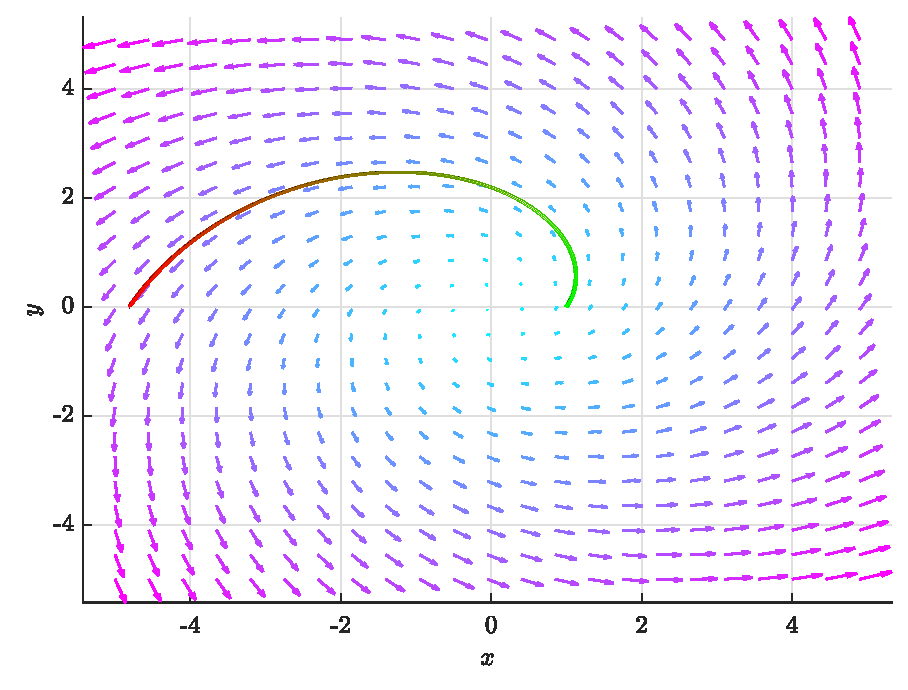
\includegraphics[width=.6\textwidth]{figures/flow}   
\end{figure}
\end{enumerate}
\end{solution}
\vspace*{1cm}
\textcolor{red}{
\noindent \textbf{Rubric:}
\begin{enumerate}[(a)]
    \item \textbf{(1 pt.)} Attempt to write as linear system $\vecxdot(t) = [A(t)] \vecx$. \textbf{(1 pt.)} Correct matrix $[A]$.
    \item \textbf{(1/2 pt.)} Correct $\vecxdot$. \textbf{(1/2 pt.)} Correct $\vecfieldV(\vecx)$. \textbf{(1 pt.)} Show that the two are equal.
	\item \textbf{(1 pt.)} Correct particular solution.
    \item \textbf{(1 pt.)} Plot of $\vecfieldV$. \textbf{(1 pt.)} Plot of solution.
\end{enumerate}
}

\newpage
\begin{problem}
\textbf{(7 pts.)} Consider our model for a molecular crystal potential for which we took the scalar field
\[
u(x,y)=\cos^2(x)+\cos^2(y).
\]
\begin{enumerate}[(a)]
\item \textbf{(1 pts.)} Plot the graph of of $u(x,y)$ and the level curves. Feel free to use your old work.
\item \textbf{(1 pts.)} Write down the differential equation for a curve given by gradient descent of the system. That is, the negative of the gradient flow. 
\item \textbf{(2 pts.)} Without solving the problem, where would particles end up if they follow gradient descent? What if particles start on a peak?
\item \textbf{(3 pts.)} Recall the matrix $[J]$ given by
\[
[J] = \begin{pmatrix} 0 & -1 \\ 1 & 0 \end{pmatrix}.
\]
The \emph{Hamiltonian flow} is given by
\[
\boldsymbol{\dot{\vec{x}}}(t) = [J] \grad u(\vecx(t)).
\]
The \emph{Hamiltonian vector field} is the right hand side,
\[
[J] \grad u(x,y).
\]
Plot the Hamiltonian vector field and explain why the level curves to $u(x,y)$ correspond to the Hamiltonian flows.
\end{enumerate}
\end{problem}
\begin{solution}~
\begin{enumerate}[(a)]
\item Here are the plots for the graph of $u(x,y)$ as well as the level curves.
    \begin{figure}[H]
    	\centering
        \begin{subfigure}[b]{0.45\textwidth}
        \centering
    	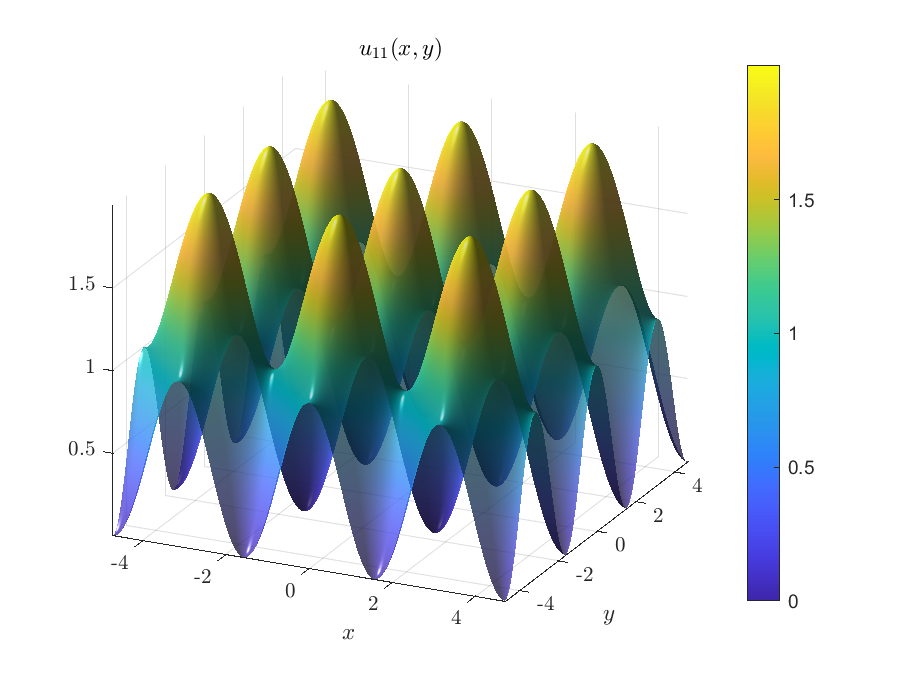
\includegraphics[width=\textwidth]{figures/crystal_surface}
        \caption{Graph of $u(x,y)$.}
        \end{subfigure}
\hfill
        \begin{subfigure}[b]{0.45\textwidth}
        	\centering
        	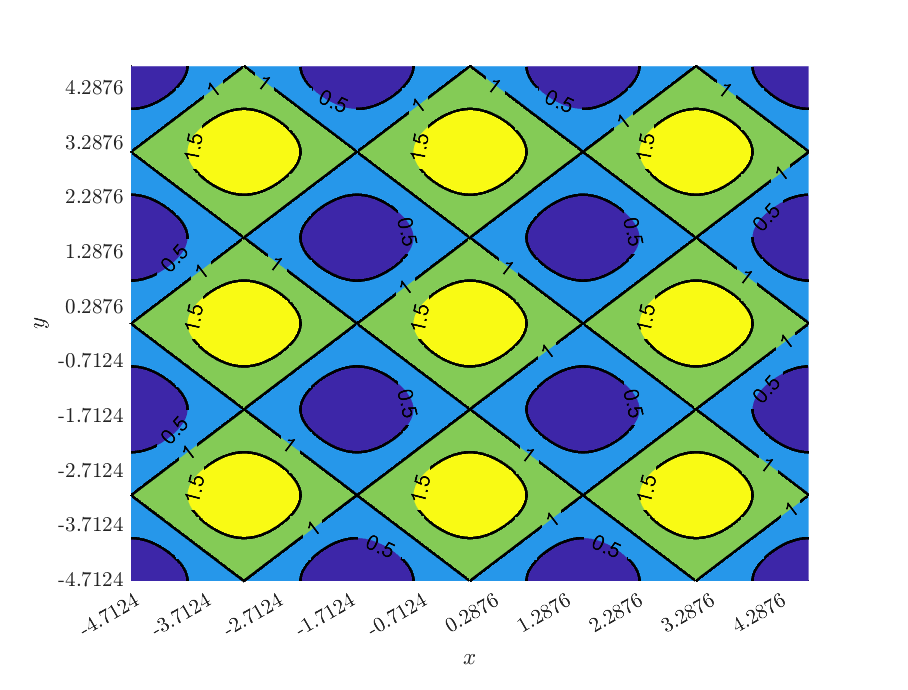
\includegraphics[width=\textwidth]{figures/level_curves}
            \caption{Level curves to $u(x,y)$.}
        \end{subfigure}
\end{figure}
\item First, we have
\[
\grad u = \begin{pmatrix} -2 \cos(x)\sin(x)\\ -2 \cos(y)\sin(y) \end{pmatrix}
\]
Hence, the negative gradient flow is
\begin{align*}
	\vecxdot(t) &= - \grad u(\vecx(t))\\
	\begin{pmatrix} \dot{x}(t) \\ \dot{y}(t)\end{pmatrix} &= \begin{pmatrix} 2 \cos(x(t))\sin(x(t))\\ 2 \cos(y(t))\sin(y(t)) \end{pmatrix}
\end{align*}

\item Negative gradient ascent will tell the particle to flow downhill hence, almost always, the particle will end up at the local minimas (i.e., the valleys of the surface shown in (a)). These minima occur at
\[
(x,y)=\left( 2\pi m \pm \frac{\pi}{2}, 2 \pi n \pm \frac{\pi}{2} \right)
\]
for integers $m$ and $n$. 

The only time this may not happen is when a particle begins at a maxima which are
\[
(x,y)=\left( \pi m , \pi n \right).
\]
In that case, the gradient is zero so the particle will not move. The other odd case will be if a particle starts on a ridge between two peaks. Then the particle may not end up in a valley. 

In fact, here is a plot of the gradient flow lines.
\begin{figure}[H]
	\centering
	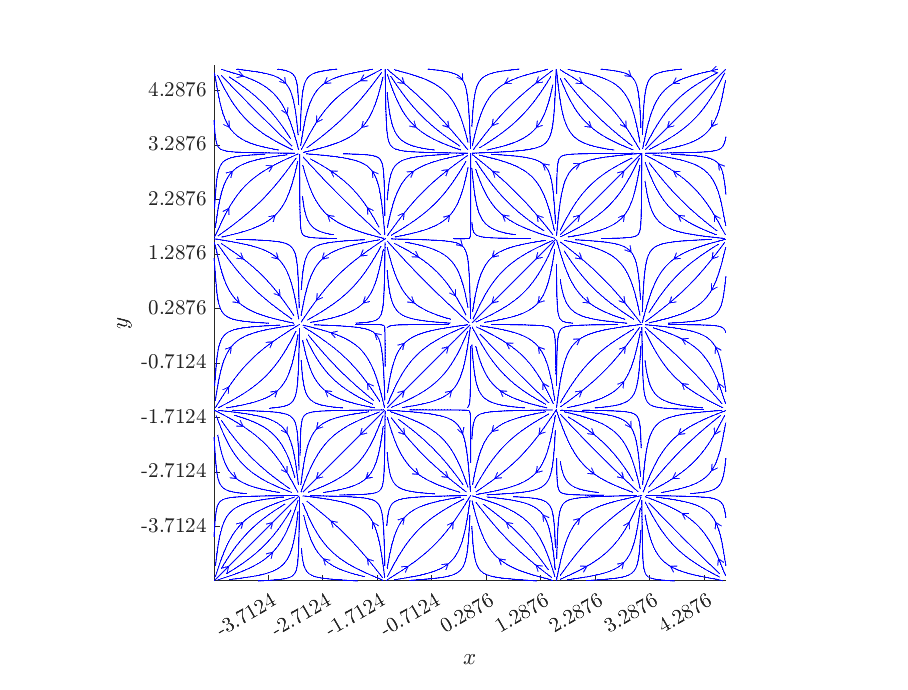
\includegraphics[width=.75\textwidth]{figures/gradient_flow}
\end{figure}

\item The Hamiltonian flow is
\begin{align*}
	\vecxdot(t) &= [J]\grad u(\vecx(t))\\
	\begin{pmatrix} \dot{x}(t) \\ \dot{y}(t)\end{pmatrix} &= \begin{pmatrix} -2 \cos(y(t))\sin(y(t))\\ 2 \cos(x(t))\sin(x(t)) \end{pmatrix}
\end{align*}
and we can see the Hamiltonian vector field and some flow streamlines like this:
    \begin{figure}[H]
    	\centering
        \begin{subfigure}[b]{0.45\textwidth}
        \centering
    	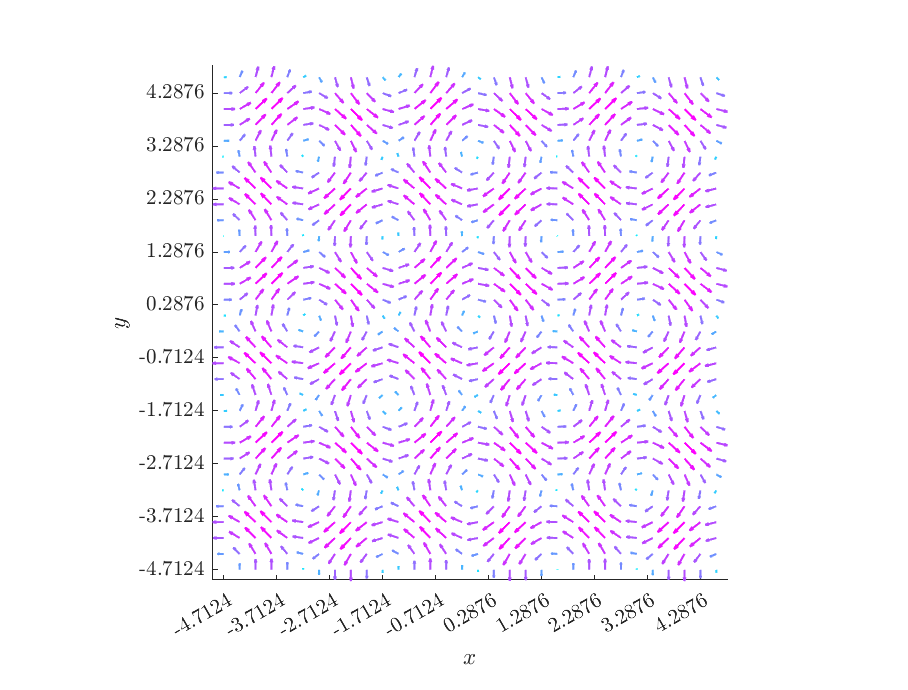
\includegraphics[width=\textwidth]{figures/hamiltonian_vec_field}
        \caption{The Hamiltonian vector field $[J]\grad u$.}
        \end{subfigure}
\hfill
        \begin{subfigure}[b]{0.45\textwidth}
        	\centering
        	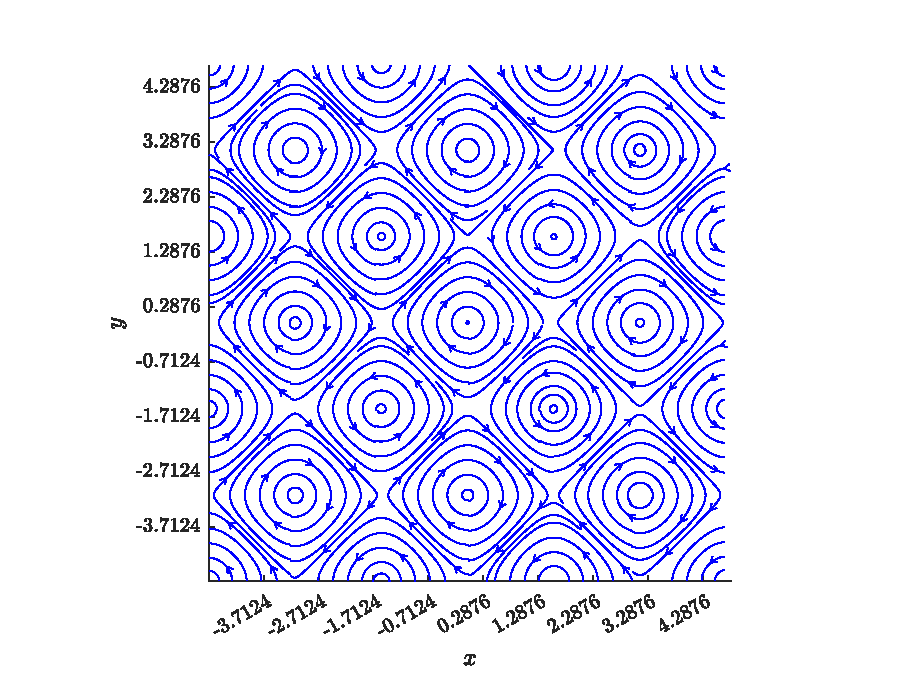
\includegraphics[width=\textwidth]{figures/hamiltonian_flow}
            \caption{Flows of the Hamiltonian vector field.}
        \end{subfigure}
\end{figure}
The reason why the level curves are flows of the Hamiltonian field is that the gradient $\grad u$ is always perpendicular to the level curves. So, the gradient flow flows directly through the level curves. However, the matrix $[J]$ is a rotation matrix that rotates by $\pi/2$, so the Hamiltonian vector field $[J]\grad u$ is parallel to the level curves. Hence, the flows of the Hamiltonian vector field must stay on the level curves.
\end{enumerate}
\end{solution}
\vspace*{1cm}
\textcolor{red}{
\noindent \textbf{Rubric:}
\begin{enumerate}[(a)]
    \item \textbf{(1/2 pt.)} Correct graph of surface. \textbf{(1/2 pt.)} Correct level curves.
    \item \textbf{(1 pt.)} Correct equation.
	\item \textbf{(1 pt.)} Mention of particles flowing towards the minimas (valleys/troughs). \textbf{(1 pt.)} Explaining that particles at the top of a peak will not move over time.
    \item \textbf{(1 pt.)} Correct Hamiltonian vector field. \textbf{(1 pt.)} Plot of Hamiltonian vector field. \textbf{(1 pt.)} Explanation of why the flows are the level curves of $u$.
\end{enumerate}
}

\newpage

\begin{problem}
\textbf{(10 pts.)} Let us consider the discrete heat equation for $n$ equally spaced particles on a line segment for which we have the following picture
\begin{figure}[H]
	\centering
	\resizebox{.9\columnwidth}{!}{\input{figures/equally_spaced_line_points.pdf_tex}}
\end{figure}
Let $u_j(t) \coloneqq u(x_j,t)$ denote the temperature of particle $j$ at time $t$, let $k_j$ be the thermal transport coefficient between particles $j$ and $j+1$, and let $f_j(t)=f(x_j,t)$ be the thermal energy source on particle $j$.
\begin{enumerate}[(a)]
    \item \textbf{(2 pts.)} For the boundary particles $x_1$ and $x_n$, we have
    \[
    \dot{u}_1 = -k_1 u_1 + k_1 u_{2} + f_1 \qquad \textrm{and} \qquad \dot{u}_n = -k_n u_{n} + k_{n-1} u_{n-1} +f_n,
    \]
    which correspond to \emph{Neumann type boundary conditions}. Explain each term in the above equations.
    \item \textbf{(2 pts.)} If we attached $x_1$ to $x_n$ with a material with a thermal transport coefficent of $k_0$ the above equations would need modification. Write these new equations. These are the \emph{periodic boundary conditions}. 
    \item \textbf{(1 pts.)} Explain why periodic boundary conditions are the same as working with a circular domain.
    \item \textbf{(1 pts.)} If we force $u_1$ and $u_n$ to be constant, what will the equations for the boundary particles be? These would be the \emph{Dirichlet type boundary conditions}.
    \item \textbf{(2 pts.)} For the interior particles, we have the relationship
    \[
    \dot{u}_j = -k_{j-1}u_j - k_{j} u_j + k_{j-1}u_{j-1} + k_{j} u_{j+1} +f_j \qquad \textrm{for $j=2,\dots,n-1$}.
    \]
    Explain what each term describes in the above equation.
    \item \textbf{(2 pts.)} In the limit as $n\to \infty$, we then have that $k$ is described as a function of position, $x$. The source free heat equation then reads
    \[
    \frac{\partial}{\partial t}u(x,t) = \frac{\partial}{\partial x} \left( k(x)\frac{\partial}{\partial x} u(x,t) \right) + f(x,t).
    \]
    Explain how this equation differs from the equation
    \[
    \frac{\partial}{\partial t}u(x,t) = k(x) \frac{\partial^2}{\partial x^2} u(x,t)+f(x,t).
    \]
\end{enumerate}
\end{problem}
\begin{solution}~
\begin{enumerate}[(a)]
    \item Let us concentrate on the two terms that appear in the first equation
    \[
\dot{u}_1 = \underbrace{-k_1 u_1}_{1} \underbrace{+ k_1 u_{2}}_{2}\underbrace{+f_1}_5.
    \]
    The rate of change of the temperature of particle 1, $\dot{u}_1$, depends on these three terms. For term 1, this corresponds to thermal energy leaving particle 1 at a rate given by the thermal transport coefficient $k_1$ and proportional to the temperature of particle $1$, $u_1$. Term 2 is the thermal energy entering particle 1 given by particle 2 at a rate $k_1$ proportional to the temperature of particle 2, $u_2$. The rates here are all the same since the two particles are connected by the same media. Thus, the rate of change of particle 1 can also be written as
    \[
    \dot{u}_1 = k_1(u_2-u_1) +f_1,
    \]
    which is equivalent to Newton's law of cooling with an additional heat source due to $f_1$. That is, the rate of change of temperature of a body is proportional to the difference of the temperature of the body and its surroundings in the case where the source term $f_1=0$. Term 3, $+f_1$, describes the rate of heat energy being added to particle 1. The equation for particle $n$ is completely analogous.

    \item The equations we have will need an additional term that corresponds to thermal transport to the particle at the other end of the interval. The original terms remain. Thus, we would have
    \[
\dot{u}_1 = -k_1 u_1 + k_1 u_{2} -k_0 u_1  + k_0 u_n+ f_1 \qquad \textrm{and} \qquad \dot{u}_n = -k_n u_{n} + k_1 u_{n-1} - k_0 u_n + k_0u_1 f_n.
    \]
    
    \item The above equations go to show that we have added medium between particles 1 and 2 so that 1 and 2 are in thermal contact. Thus, it is sensible to realize that we have taken this line of particles and attached endpoints to form a circle.

    \item The equations in this case are quite simple. We have
    \[
    \dot{u}_1 = 0 \qquad \textrm{and} \qquad \dot{u}_n = 0.
    \]
    Hence, we must also require that $f_1=0$ and $f_n=0$.
    

    \item Let us isolate the terms in the equation
\[
\dot{u}_j = \underbrace{-k_{j-1}u_j}_1 \underbrace{- k_{j} u_j}_2 \underbrace{+ k_{j-1}u_{j-1}}_3 \underbrace{+ k_{j} u_{j+1}}_4 \underbrace{+ f_j}_5.
\]
Terms 1 and 2 are negative, which mean they correspond to thermal energy lost by particle $j$. Indeed, thermal energy will be transported to particle $j-1$ through the medium with the thermal transport coefficient $k_{j-1}$ and proportional to $u_{j}$ (term 1) and thermal energy will transport to particle $j+1$ via the media with $k_j$ and proportional to $u_j$ (term 2). Terms 3 and 4 are positive, so they correspond to thermal energy gained by particle $j$. Particle $j$ receives thermal energy from particle $j-1$ via $k_{j-1}u_{j-1}$ and from particle $j+1$ via $k_j u_{j+1}$. Finally, term 5 is again the rate of thermal energy being added to particle $j$.

\item In the first equation, we have a product rule to apply to yield
\[
\frac{\partial}{\partial x} \left( k(x)\frac{\partial}{\partial x} u(x,t) \right) = \frac{d k}{dx} \frac{\partial u}{\partial x} + k \frac{\partial^2 u}{\partial x^2}.
\]
Indeed, this means that there is an extra term when we compare to the second equation. This term deals with the fact that the thermal transport medium itself can vary from point to point, and the gradient of this adds additional changes the diffusion process.
\end{enumerate}
\end{solution}
\vspace*{1cm}
\textcolor{red}{
\noindent \textbf{Rubric:}
\begin{enumerate}[(a)]
    \item \textbf{(1 pt.)} Explanation of $u$ and $\dot{u}$. \textbf{(1 pt.)} Explanation of $k$ and $f$ terms.
	\item \textbf{(1 pt.)} New equations for $\dot{u}_1$ and $\dot{u}_n$ include $k_0$ and the new $u_1$ or $u_n$ term. \textbf{(1 pt.)} New equations are correct.
    \item \textbf{(1 pt.)} Explain or draw a picture showing that we have now connected particle $x_1$ to particle $x_n$ and formed a circle.
	\item \textbf{(1 pt.)} Correct equations.
	\item  \textbf{(1 pt.)} Explanation of $u$ and $\dot{u}$. \textbf{(1 pt.)} Explanation of $k$ and $f$ terms.
	\item  \textbf{(1 pt.)} Explaining how the product rule makes the equations mathematically different. \textbf{(1 pt.)} Brief explanation explaining that we must care about how $k(x)$ changes as well.
\end{enumerate}
}

\newpage

\begin{problem}
    \textbf{(8 pts.)} Consider the 1-dimensional homogeneous Laplace equation given by 
    \[
    \frac{\partial^2}{\partial x^2} u_E(x) = 0,
    \]
    with the domain $\Omega$ as the unit interval on the $x$-axis.  Take the Dirichlet boundary conditions $u_E(0)=T_0$ and $u_E(L)=T_L$.  Think of these values as the ambient temperature at the endpoints of the rod.  These temperatures are constant since the ambient environment is so large.

    \begin{enumerate}[(a)]
        \item \textbf{(2 pts.)} Find the particular solution to this Laplace equation.
        \item \textbf{(2 pts.)} Suppose that $v(x,t)$ is a solution to the 1-dimensional source free isotropic heat equation with zero Dirichlet boundary values. Show that 
        \[
        u(x,t)=v(x,t)+u_E(x),
        \]  
        is a solution to the 1-dimensional source free isotropic heat equation with Dirichlet boundary values $u(0,t)=T_0$ and $u(L,t)=T_L$.
        \item \textbf{(2 pts.)} From the previous part we know that $\lim_{t\to \infty} v(x,t) = 0$.  Hence, show that the long time limit of a solution to the source free heat equation yields a solution to the Laplace equation.
        \item \textbf{(2 pts.)} Argue why the equilibrium temperature profile of a rod can be found without solving the heat equation.
    \end{enumerate}
\end{problem}
\begin{solution}~
\begin{enumerate}[(a)]
    \item Note that we can integrate this equation twice to get a general solution
    \[
    u_E(x) = ax+b.
    \]
    Now, by matching boundary conditions, we have
    \[
    T_0=u_E(0) = b,
    \]
    so $b=T_0$. The other condition gives
    \[
    T_L = u_E(L) = aL+T_0,
    \]
    thus we have $a= \frac{T_L-T_0}{L}$. This means our particular solution is
    \[
    \boxed{    u_E(L) = \frac{T_L-T_0}{L}x - T_0.}
    \]
    
    \item First, we need to see if $u=v+u_E$ is a solution to the PDE.  If we plug this in, we have
    \begin{align*}
    \left( -k\frac{\partial^2}{\partial x^2} + \frac{\partial}{\partial t} \right) u &= \left( -k\frac{\partial^2}{\partial x^2} + \frac{\partial}{\partial t} \right)(v+u_E)\\
    &= \left( -k\frac{\partial^2}{\partial x^2} + \frac{\partial}{\partial t} \right)v(x,t) + \left( -k\frac{\partial^2}{\partial x^2} + \frac{\partial}{\partial t} \right)u_E(x).
    \end{align*}
    Now, note that
    \[
    \left( -k\frac{\partial^2}{\partial x^2} + \frac{\partial}{\partial t} \right)v(x,t) = 0,
    \]
    since we stated $v$ is a solution to this equation and note
    \[
    \left( -k\frac{\partial^2}{\partial x^2} + \frac{\partial}{\partial t} \right)u_E(x) = 0
    \]
    since $u_E(x)$ doesn't depend on $t$ and $u_E(x)$ solves the Laplace equation.
    
    Finally, we need to show that $u=v+u_E$ satisfies the boundary conditions.  Since $v(0,t)=0=v(L,t)$ by our supposition, we have that $u(0,t)=u_E(0)=T_0$ and $u(L,t)=u_E(L)=T_L$. Thus $u(x,t)$ is indeed a solution to the boundary value problem.
    
    \item We can take
    \[
    \lim_{t\to \infty} u(x,t) = \lim_{t\to \infty} \left( v(x,t) + u_E(x) \right) = u_E(x),
    \]
    which shows that $u_E(x)$ is the equilibrium temperature profile.  This is also the solution to the Laplace equation!
    
    \item To find the equilibrium temperature profile, we just needed to solve the Laplace equation.  That was the argument we made in (c). The equilibrium does not depend on time, since it is the result of waiting for $t\to \infty$. So, determining this is a completely separate problem if we wish it to be!
\end{enumerate}
\end{solution}
\textcolor{red}{
\noindent \textbf{Rubric:}
\begin{enumerate}[(a)]
    \item \textbf{(1 pt.)} Correct general solution. \textbf{(1 pt.)} Applied boundary conditions and got correct particular solution.
	\item \textbf{(1 pt.)} Show the solution $u$ solves the PDE. \textbf{(1 pt.)} Show that $u$ also satisfies the boundary conditions.
    \item \textbf{(1 pt.)} Take the limit to remove $v(x,t)$ \textbf{(1 pt.)} Explain that $u_E$ is what's leftover and it solves the Laplace equation.
	\item \textbf{(1 pt.)} Mention the argument in (c). \textbf{(1 pt.)} Given that, an explanation on why we can just solve the Laplace equation. 
\end{enumerate}
}

\newpage
\begin{problem}
    \textbf{(3 pts.)} Using intuition from the previous problem, explain how one could solve the heat equation with a nonzero source term that only depends on $x$. In other words, how could one try to solve
    \[
    \left( -k \frac{\partial^2}{\partial x^2} + \frac{\partial}{\partial t} \right) u(x,t) = f(x),
    \]
\end{problem}
\begin{solution}
One could argue that the equilibrium solution $u_E(x)$ will solve the equation
\[
-k\frac{\partial^2}{\partial x^2} u_E(x) = f(x),
\]
since this mimics what we did in the earlier problem.  This shows that when there are sources of heat in the material, they will contribute to the equilibrium temperature profile. How so? Take $u(x,t)=v(x,t)+u_E(x)$ as before, then
\begin{align*}
\left( -k \frac{\partial^2}{\partial x^2} + \frac{\partial}{\partial t} \right) u(x,t) &= f(x)\\
\left( -k \frac{\partial^2}{\partial x^2} + \frac{\partial}{\partial t} \right)( v(x,t)+u_E(x)) &= f(x)\\
\left( -k \frac{\partial^2}{\partial x^2} + \frac{\partial}{\partial t} \right) v(x,t) + -k \frac{\partial^2}{\partial x^2} u_E(x) &= f(x),
\end{align*}
and since $v(x,t)$ solves the 1d heat equation, are left with the above equation (\cref{eq:poisson}). Moreover, one should note that the boundary conditions must be handled by $u_E(x)$ as in problem 3.
\end{solution}
\textcolor{red}{
\noindent \textbf{Rubric:}
\begin{enumerate}[(a)]
    \item \textbf{(1 pt.)} Consider the ansatz $u(x,t)=v(x,t)+u_E(x)$. \textbf{(1 pt.)} Use the ansatz to show $u_E(x)$ solves a Poisson equation with $f(x)$ as the right hand side. \textbf{(1 pt.)} Reasonable discussion based on previous problem.
\end{enumerate}
}
\newpage

\begin{problem}
    \textbf{(13 pts.)} Consider the 2-dimensional source free isotropic heat equation given by
    \[
    \left( -k \Delta + \frac{\partial}{\partial t} \right) u(x,y,t) = 0,
    \]
    with the domain $\Omega$ as the unit square in the $xy$-plane. Take as well the Dirichlet boundary conditions $u(x,y,t)=0$ for $x$ and $y$ on the boundary of $\Omega$.
    \begin{enumerate}[(a)]
        \item \textbf{(2 pts.)} Show that $u_{mn}(x,y,t)=\sin(m\pi x)\sin(n\pi y)e^{-k(n^2+m^2)\pi^2 t}$ is a solution to the PDE and Dirichlet boundary conditions for any non-negative integers $m$ and $n$.
        \item \textbf{(2 pts.)} Show that a linear combination of solutions $u_{mn}$ and $u_{pq}$ is also a solution.
        \item \textbf{(3 pts.)} For $m=n=1$ and $k=1$, plot the solution for the values $t=0$, $t=0.01$, $t=0.1$ and $t=1$.  Explain what is physically happening as time moves forward.
        \item \textbf{(2 pts.)} Explain what varying the value for the conductivity $k$ does to the solution.  Feel free to use plots to support your hypothesis.
        \item \textbf{(2 pts.)} Explain the mathematical reason why increasing $m$ and $n$ causes the solution to converge to zero more quickly.
        \item \textbf{(2 pts.)} Explain the physical reason why increasing $m$ and $n$ causes the solution to converge to zero more quickly. Plots may help support your reasoning.
    \end{enumerate}
\end{problem}
\begin{solution}~
\begin{enumerate}[(a)]
    \item We can simply take the necessary derivatives to show that $u_{mn}$ is a solution.  We have
    \begin{align*}
    -k\Delta u_{mn} &= -ke^{-k(m^2+n^2)\pi^2 t} \left( -m^2\pi^2 \sin(m\pi x)\sin(n\pi y)-n^2\pi^2 \sin(m\pi x)\sin(n\pi y)\right) \\
    &=k(m^2+n^2)\pi^2 u_{mn}
    \end{align*}
    Then we also have
    \[
    \frac{\partial}{\partial t} u_{mn} = -k(m^2+n^2)\pi^2 u_{mn}.
    \]
    Hence, if we add these two together we have
    \[
    -k\Delta u_mn + \frac{\partial}{\partial t} u_{mn} = 0.
    \]
    So $u_{mn}(x,y,t)$ is a solution to the PDE for all $m$ and $n$.
    
    Now, as far as the boundary conditions go, the boundary to $\Omega$ is broken into four pieces
    \begin{align*}
    x\in [0,1] ~\& ~ y=0\\
    x\in [0,1] ~\& ~ y=1\\
    y\in [0,1] ~\& ~ x=0\\
    y \in [0,1] ~\& ~ x=1.
    \end{align*}
    Note that when $x=0$ or $x=1$, we have $\sin(m\pi x)=0$ since $m$ is an integer. Similarly we have for $y=0$ or $y=1$ that $\sin(n\pi y)=0$.  Thus, $u_{mn}=0$ along the boundary.
    
    \item Take $u=\alpha_{mn}u_{mn}+\alpha_{pq}u_{pq}$.  Then
    \begin{align*}
        \left( -k \Delta + \frac{\partial}{\partial t} \right) u &= \left( -k \Delta + \frac{\partial}{\partial t} \right)(\alpha_{mn}u_{mn} + \alpha_{pq} u_{pq} )\\
        &= \alpha_{mn} \left( -k \Delta + \frac{\partial}{\partial t} \right)u_{mn} + \alpha_{pq} \left( -k \Delta + \frac{\partial}{\partial t} \right) u_{pq}\\
        &=0,
    \end{align*}
    since $u_{mn}$ and $u_{pq}$ are solutions.
    
    \item Here are the plots
    \begin{figure}[H]
    	\centering
        \begin{subfigure}[b]{0.3\textwidth}
        \centering
    	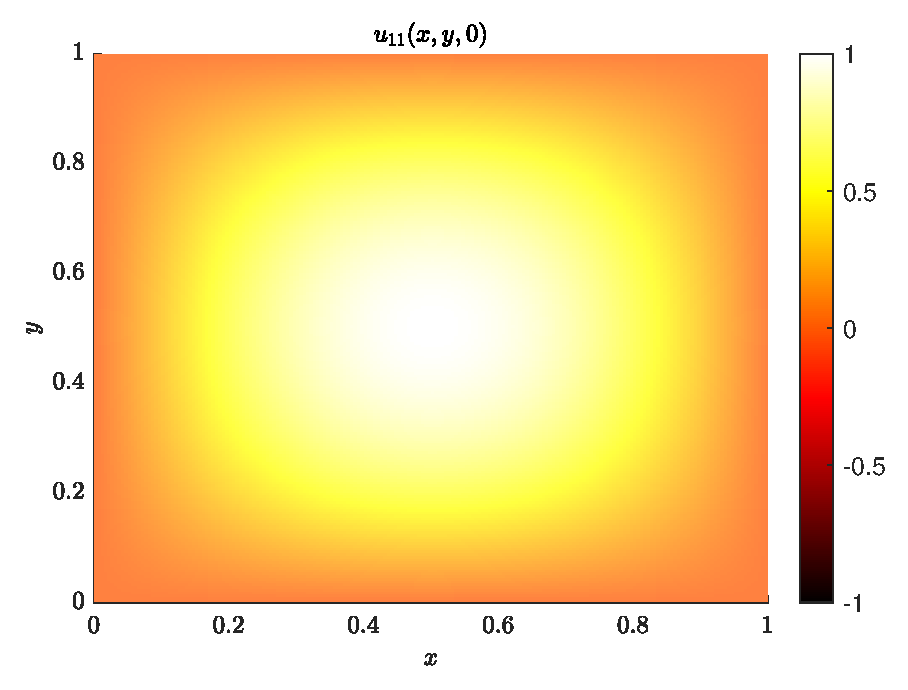
\includegraphics[width=\textwidth]{figures/heat_solution_t=0}
        \caption{Solution at $t=0$.}
        \end{subfigure}
\hfill
        \begin{subfigure}[b]{0.3\textwidth}
        	\centering
        	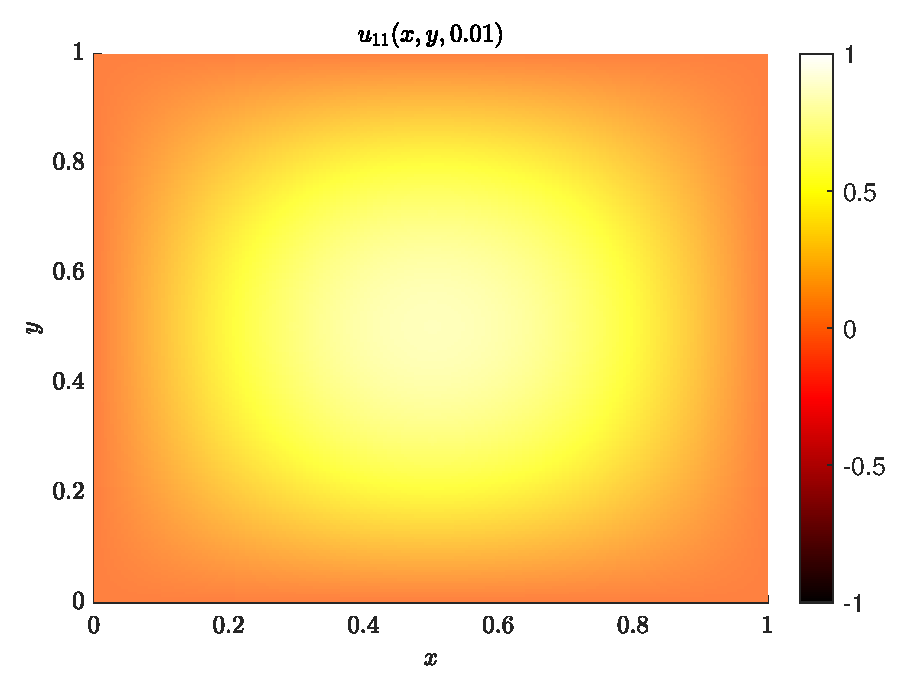
\includegraphics[width=\textwidth]{figures/heat_solution_t=0.01}
            \caption{Solution at $t=0.01$.}
        \end{subfigure}
\hfill
        \begin{subfigure}[b]{0.3\textwidth}
        	\centering
        	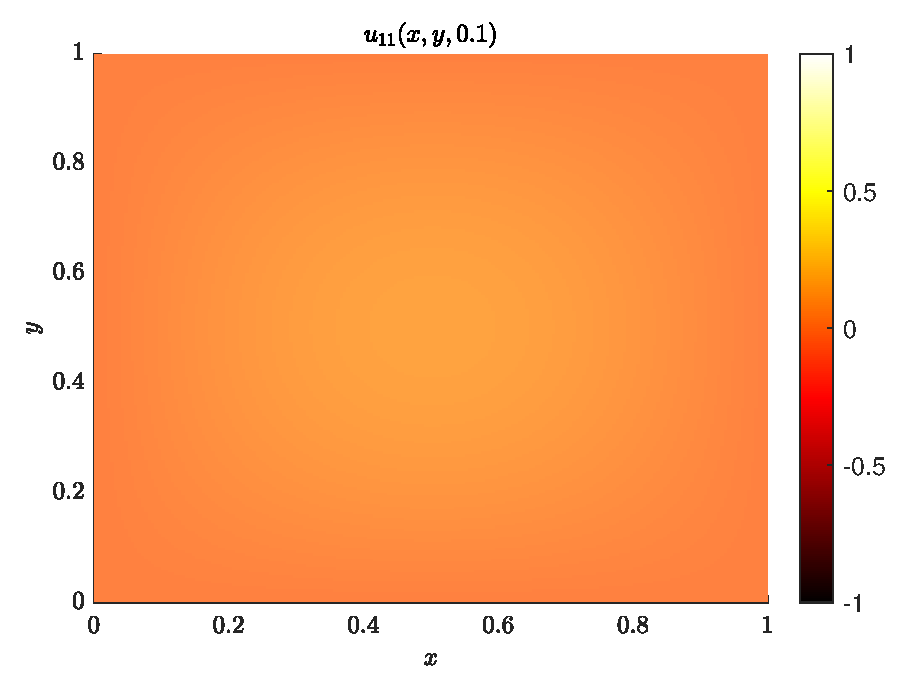
\includegraphics[width=\textwidth]{figures/heat_solution_t=0.1}
            \caption{Solution at $t=0.1$.}
        \end{subfigure}
\caption{The color displays the temperature as shown by the colorbar.}
\end{figure}
    As time moves forward, we find that the plate is cooling down to the temperature of the boundary.  So, the whole plate will reach a temperature of zero if we go indefinitely far in the future.
    
    \item $k$ decides how quickly heat will flow in our material. Larger values of $k$ means that temperature will flow more easily.  We can see this in the equation since a larger $k$ will make the exponential decay term in our equation approach zero more rapidly.  One can also repeat the plots in the previous part but for a larger value of $k$ to see this in action.
    
    \item The mathematical reason why is similar to what we discussed in the previous part.  If we increase $m$ or $n$, we find that the exponential decay happens at a quicker rate.
    
    \item Physically, as $m$ and $n$ increase, we have more hot and cold regions placed next to each other.  When there are two regions of vastly different temperature close to each other, they will equilibrate more quickly.  These two plots show what this looks like pictorially.
    \begin{figure}[H]
            \begin{subfigure}[b]{0.45\textwidth}
            	\centering
            	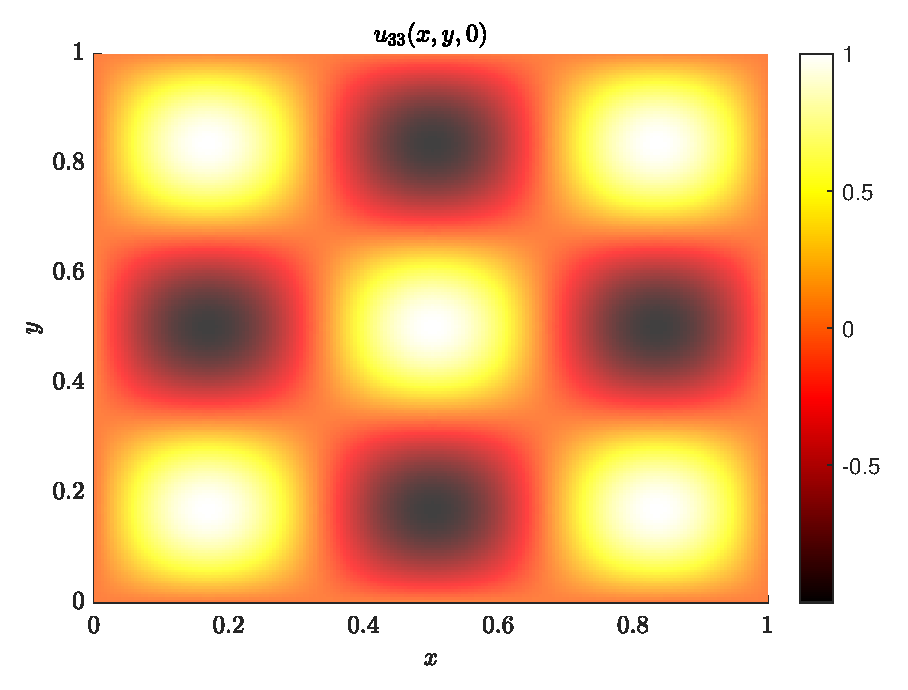
\includegraphics[width=\textwidth]{figures/heat_solution_m=3_n=3}
                \caption{At $t=0$, this is the profile for $m=3$ and $n=3$.}
            \end{subfigure}
\hfill
            \begin{subfigure}[b]{0.45\textwidth}
            	\centering
                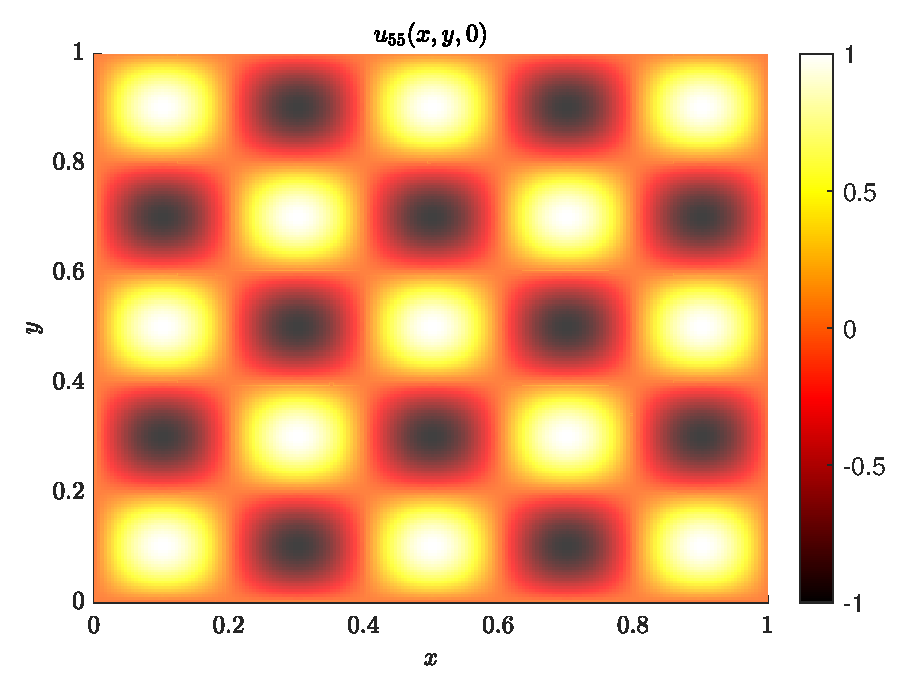
\includegraphics[width=\textwidth]{figures/heat_solution_m=5_n=5}
                \caption{At $t=0$, this is the profile for $m=5$ and $n=5$.}
            \end{subfigure}
\caption{The color displays the temperature as shown by the colorbar.}
        \end{figure}
\end{enumerate}
\end{solution}
\textcolor{red}{
\noindent \textbf{Rubric:}
\begin{enumerate}[(a)]
    \item \textbf{(1 pt.)} Show it satisfies PDE. \textbf{(1 pt.)} Show it satisfies boundary conditions. 
	\item \textbf{(1 pt.)} Correct idea for a linear combination. \textbf{(1 pt.)} Correct work to show the linear combination is a solution.
	\item \textbf{(1 pt.)} Correct plot for $t=0$. \textbf{(1 pt.)} Reasonable looking graphs for $t=0$ and $t=0.01$. \textbf{(1 pt.)} Correct argument for what happens as time increases.
	\item \textbf{(1 pt.)} Argues larger $k$ will make the solution decay faster. \textbf{(1 pt.)} Some type of evidence for the claim (plot or math).
	\item \textbf{(1 pt.)} Mention of the appearance of $m$ and $n$ in the exponent. \textbf{(1 pt.)} Reasoning that a larger negative exponent decreases more quickly.
	\item \textbf{(1 pt.)} Mention that hot and cold spots become closer to each other. \textbf{(1 pt.)} Mention that because hot and cold spots are closer, heat is transported more quickly between them.
\end{enumerate}
}

\newpage
\begin{problem}
\textbf{(11 pts.)} Consider the 1-dimensional wave equation given by
\[
\left(-\frac{\partial^2}{\partial x^2} +\frac{1}{c^2} \frac{\partial^2}{\partial  t^2} \right) u(x,t) = 0.
\]
We'll consider two distinct scenarios. First, we'll take an infinitely long elastic rod and second we'll take a rod of finite length with Dirichlet boundary conditions.
\begin{enumerate}[(a)]
    \item \textbf{(2 pts.)} For a rod of infinite length, consider the initial conditions
    \[
    u(x,0) = \begin{cases} x+1 & -1\leq x \leq 0 \\ 1-x & 0\leq x \leq 1 \\ 0 & \textrm{otherwise} \end{cases} \qquad \textrm{and} \qquad \frac{\partial}{\partial t} u(x,0) = 0.
    \]
    Find and plot the portion of the wave that moves to the right with $c=1$.
    \item \textbf{(2 pts.)} Let $u_R(x,t)$ be your solution from (a), show that this satisfies the right-moving wave equation
    \[
    \left(\frac{\partial}{\partial x} + \frac{1}{c} \frac{\partial}{\partial t} \right)u_R(x,t) = 0.
    \]
    \item \textbf{(1 pts.)} Why is it that we can ignore the points where your function $u_R(x,t)$ is not differentiable even though we are considering this as a solution to a PDE?
    \item \textbf{(2 pts.)} For an elastic rod $\Omega$ of finite length, $\Omega = [0,1]$, assume that we take the Dirichlet conditions $u(0,t)=0=u(1,t)$.  With the initial conditions
    \[
    u(x,0) = \sin(\pi x) \qquad \textrm{and} \qquad \frac{\partial}{\partial t} u(x,0)=0,
    \]
    find the solution using d'Alembert's formula.
    \item \textbf{(2 pts.)} Let $w(x,t)$ be your solution for (d), show that it is indeed equal to
    \[
    w(x,t) = \sin(\pi x)\cos(\pi c t).
    \]
    \item \textbf{(2 pts.)} With your result from (e), explain how we can decompose a standing wave into a linear combination of two waves; one moving towards the left and one moving towards the right and both reflecting off the boundary.
\end{enumerate}
\end{problem}
\begin{solution}~
\begin{enumerate}[(a)]
    \item We have that the solution is given by
\[
u(x,t) = \frac{1}{2} \left( u_L(x,t) + u_R(x,t)\right),
\]
where $u_L(x,t)$ is a portion of the wave moving to the left and $u_R(x,t)$ is the portion of the wave moving towards the right.  From our initial conditions, we have
\[
u_L(x,t) = \begin{cases} x+ct+1 & -1\leq x+ct \leq 0 \\ 1-x-ct & 0\leq x+ct \leq 1 \\ 0 & \textrm{otherwise} \end{cases} \qquad \textrm{and} \qquad u_R(x,t)=\begin{cases} x-ct+1 & -1\leq x-ct \leq 0 \\ 1-x+ct & 0\leq x-ct \leq 1 \\ 0 & \textrm{otherwise} \end{cases},
\]
which follows from d'Alembert's formula. 

We can then plot $u_R(x,t)$ for a few different times with $c=1$. 
\begin{figure}[H]
    \centering
    \includegraphics[width=.8\textwidth]{figures/right_moving_triangle.png}
    \caption{Plots of $u_R$ for $t=0$ (green), $t=1/2$ (blue), $t=1$ (purple), $t=2$ (red), and $t=4$ (orange).}
\end{figure}
    \item We can take the derivatives of $u_R(x,t)$ to get
    \[
    \frac{\partial}{\partial x} u_R(x,t) = \begin{cases} 1 & -1< x-ct < 0 \\ -1 & 0<x-ct < 1 \\ 0 & \textrm{otherwise} \end{cases}
    \]
    as well as
    \[
    \frac{1}{c}\frac{\partial}{\partial t} u_R(x,t) = \frac{1}{c}\begin{cases} -c & -1< x-ct < 0 \\ c & 0<x-ct < 1 \\ 0 & \textrm{otherwise} \end{cases}.
    \]
    Then, if we add the two together, we get our intended result
    \[
    \left(\frac{\partial}{\partial x} + \frac{1}{c} \frac{\partial}{\partial t} \right)u_R(x,t) = 0
    \]
    Notice, this is true aside from the three points where we see the kinks in our wave.
    
    \item The function may not be differentiable at three distinct $x$ values for every time $t$, but this is fairly unimportant.  Roughly speaking, we can choose to ignore three points in which we have issues since this works on infinitely many other points.  There is more detail here, but that is mathematics left to discover for yourself on a later day.
    
    \item From d'Alembert's formula we see that
    \[
    u_L(x,t) = \sin(\pi (x+ct)) \qquad \textrm{and} \qquad u_R(x,t) = \sin(\pi (x-ct)).
    \]
    Hence, our solution is given by
    \[
    u(x,t) = \frac{1}{2} \left(\sin(\pi (x+ct))+\sin(\pi(x-ct))\right).
    \]
    
    \item Note that we have the trigonometric identity
    \[
    \sin(a+b) = \sin(a)\cos(b)+\cos(a)\sin(b).
    \]
    Applying this to $u_L$ and $u_R$ we have
    \[
    u_L(x,t) = \sin(\pi x+\pi ct) = \sin(\pi x)\cos(\pi c t)+ \cos(\pi x)\sin(\pi c t),
    \]
    and
    \[
    u_R(x,t) = \sin(\pi x-\pi ct) = \sin(\pi x)\cos(-\pi c t)+ \cos(\pi x)\sin(-\pi c t).
    \]
    Then, we have
    \begin{align*}
        u(x,t) &= \frac{1}{2} \left(\sin(\pi x)\cos(\pi c t)+ \cos(\pi x)\sin(\pi c t) + \sin(\pi x)\cos(-\pi c t)+ \cos(\pi x)\sin(-\pi c t) \right)\\
        &= \frac{1}{2} \left( \sin(\pi x)\cos(\pi c t) + \sin(\pi x)\cos(\pi c t) + \cos(\pi x)\sin(\pi c t) - \cos(\pi x)\sin(\pi c t)\right)\\
        &= \sin(\pi x) \cos(\pi c t) = w(x,t),
    \end{align*}
    which is indeed the solution we have found to this problem previously.
    
    \item In the previous example, we took two different waves; one moving towards the left and one moving towards the right.  It turned out that adding these solutions could be cleverly combined into a single standing wave solution.  Essentially, the separation of variables seems to help us find standing waves (though it can also find traveling waves) where as the d'Alembert method decomposes waves into their portions that move in either direction naturally. 
    
    In this case, it must be that the traveling waves are reflected by the boundaries in order to produce a standing wave.  If you play with a slinky, you may be able to discover this behavior yourself!
  \end{enumerate}
\end{solution}
\textcolor{red}{
\noindent \textbf{Rubric:}
\begin{enumerate}[(a)]
    \item \textbf{(1 pt.)} Find correct $u_R$. \textbf{(1 pt.)} Plot of $u_R$ in some way.
	\item \textbf{(2 pt.)} Correct work to see that $u_R$ is a solution by working with the piecewise definition.
	\item \textbf{(1 pt.)} A reasonable explanation. Nothing precise needed.
	\item \textbf{(1 pt.)} Find correct $u_R$ and $u_L$. \textbf{(1 pt.)} Add them to get correct $u(x,t)$ (or, $w(x,t)$ as we refer to it next).
	\item \textbf{(2 pt.)} Use the correct trig identities to get the result.
	\item \textbf{(1 pt.)} Mention work in (e). \textbf{(1 pt.)} Some kind of plot or interpretation on why this works.
\end{enumerate}
}

\newpage
\begin{problem}
    \textbf{(8 pts.)} Consider the wave problem on the region $\Omega=[0,1]$ given by
    \[
    \begin{cases}
    \left( - \frac{\partial^2}{\partial x^2} +\frac{1}{c^2} \frac{\partial^2}{\partial t^2} \right) u(x,t) =0, & \textrm{in $(0,1)$},\\
    u(0,t)=0 \textrm{~and~} u(1,t)=0, &\textrm{as boundary conditions},\\
    u(x,0)=\sin(\pi x), &\textrm{as the initial condition}.
    \end{cases}
    \]
    This problem corresponds to taking a plucked elastic string fixed at the endpoints.
    \begin{enumerate}[(a)]
        \item \textbf{(1 pts.)} Use the separation of variables ansatz $u(x,t)=X(x)T(t)$ to get a new separation constant. This will give two ODEs: one will be in terms of $X(x)$ and the other will be in terms of $T(t)$.
        \item \textbf{(2 pts.)} Use the boundary conditions and solve the ODE that is in terms of $X(x)$ which will simultaneously find the allowed values for the separation constant.
        \item \textbf{(2 pts.)} Using these allowed values for the separation constant, find the solution for $T(t)$.
        \item \textbf{(1 pts.)} Find the particular solution for $u(x,t)$ by matching the initial condition.
        \item \textbf{(2 pts.)} Plot your solution for $x\in [0,1]$ and $t\in [0,\infty)$ (i.e., just plot up to a large value of $t$). In this case, compare your plots for $c=1/2$ and $c=1$.
    \end{enumerate}
\end{problem}
\begin{solution}~
\begin{enumerate}[(a)]
    \item If we take $u(x,t)=X(x)T(t)$, then plugging this into the PDE yields
    \[
    -X''T+\frac{1}{c^2} XT'' = 0.
    \]
    We can then isolate each variable on one side of the equal sign to get
    \[
    \frac{X''}{X} = \frac{1}{c^2}\frac{T''}{T}.
    \]
    Note that the left hand side depends only on $x$, whereas the right hand side depends solely on $t$. Thus, it must be that both sides equal the same constant $\lambda$. This gives us two ODEs
    \[
    X'' -\lambda X = 0 \qquad \textrm{and} \qquad T'' -c^2 \lambda T = 0.
    \]
    
    \item The boundary conditions are a spatial condition and thus we must satisfy them independent of time.  Hence, we must have that $X(0)=0$ and $X(1)=0$ so that $u(0,t)=0$ and $u(1,t)=0$ respectively.  This means that $\lambda<0$ so that we get
    \[
    X(x) = a\cos(\sqrt{-\lambda}x) +b \sin(\sqrt{-\lambda} x),
    \]
    since if $\lambda \geq 0$ we will only get constant solutions which are trivial and can't match the initial conditions or exponential solutions which can't match the boundary conditions.  Applying the boundary conditions yields that $A=0$ and $\sqrt{-\lambda}=n\pi$ for any positive integer $n$. Thus we have
    \[
    X_n(x) = a_n \sin(n\pi x), 
    \]
    is (nontrivial) a solution to this ODE for every positive integer $n$.
    
    \item Using this result for $\lambda$, we have that
    \[
    T_n(t) = b_n \sin(cn\pi t)+c_n \cos(cn\pi t),
    \]
    for every positive integer $n$.  
    
    \item Combining to get $u_n(x,t) =X_n(x)T_n(t)$, we can write
    \[
    u_n(x,t) = \left(a_n \sin(cn\pi t)+b_n \cos(cn\pi t)\right) \sin(n\pi x),
    \]
    is a general solution for each positive integer $n$.  Note that we have just renamed constants here to write this more simply.  Now, in general, a sum of these solutions is also a solution, but we have
    \[
    u(x,0)=\sin(\pi x),
    \]
    which means that $n=1$, $a_1=0$, and $b_1=1$.  All other constants $a_j$ and $b_j$ are all zero.  One can then check that our solution
    \[
    u(x,t) = \cos(c \pi t) \sin(\pi x),
    \]
    satisfies $\frac{\partial}{\partial t} u(x,0) = 0$.  
    
    \item Here are the plots for these functions. Note that in this case, we plotted the solution as a surface with one of the axes representing time.  This still just shows how the 1-dimensional elastic evolves over time. We see that when $c$ is increased, the elastic vibrates more quickly.
    
                \begin{figure}[H]
                	\centering
                	\def\svgwidth{0.6\columnwidth}
                	\input{figures/wave_solution_c=1_2.pdf_tex}
                    \caption{The graph of the solution $u(x,t)$ for $c=1/2$.}
                \end{figure}
                \begin{figure}[H]
                                	\centering
                                	\def\svgwidth{0.6\columnwidth}
                                	\input{figures/wave_solution_c=1.pdf_tex}
                                    \caption{The graph of the solution $u(x,t)$ for $c=1$.}
                                \end{figure}
\end{enumerate}
\end{solution}

\textcolor{red}{
\noindent \textbf{Rubric:}
\begin{enumerate}[(a)]
    \item \textbf{(1 pt.)} Correct ansatz to get two ODEs.
	\item \textbf{(2 pt.)} Find the correct $X(x)$ using boundary conditions.
	\item \textbf{(1 pt.)} Correct general solution for $T(t)$. \textbf{(1 pt.)} Uses separation constant to get the correct answer.
	\item \textbf{(1 pt.)} Correct match to initial condition.
	\item \textbf{(1 pt.)} Correct looking plots. \textbf{(1 pt.)} Correcct comparison of plots with different $c$ values.
\end{enumerate}
}


\newpage

\begin{problem}
\textbf{(9 pts.)} Consider the heat flow problem on the region $\Omega=[0,1]$ given by
\[
\begin{cases}
\frac{\partial}{\partial t} u(x,t) = \frac{\partial^2}{\partial x^2} u(x,t) - 1, & \textrm{in $(0,1)$},\\
u(0,t)=0 \textrm{~and~} u(1,t)=1, & \text{as boundary conditions},\\
u(x,0) = \sin\left(\pi x\right) + \frac{1}{2}(x^2+x), & \textrm{as the initial condition}.
\end{cases}
\]
This corresponds to a rod kept at fixed temperatures at the endpoints that starts with a warm center initially.
\begin{enumerate}[(a)]
    \item \textbf{(3 pts.)} As with the previous problem, take an ansatz
    \[
    u(x,t) = v(x,t) + u_E(x)
    \]
    where $v(x,t)$ solves the following problem
    \[
\begin{cases}
\frac{\partial}{\partial t} v(x,t) = \frac{\partial^2}{\partial x^2} v(x,t), & \textrm{in $(0,1)$},\\
v(0,t)=0 \textrm{~and~} v(1,t)=0, & \text{as boundary conditions}.
\end{cases}
    \]
    Find the general solution $v(x,t)$ using separation of variables. \emph{Hint: feel free to use the work in the notes (Example ``Solving the Heat Equation" and Example ``Particular Solution to the 1D Heat Equation").}

    \item \textbf{(2 pts.)} Show that for $u(x,t)$ to be a solution that
    \[
    \frac{\partial^2}{\partial x^2} u_E(x) = 1.
    \]

    \item \textbf{(2 pts.)} Find the solution $u_E(x)$ to the following problem
    \[
    \begin{cases}
    \frac{\partial^2}{\partial x^2} u_E(x) = 1, & \textrm{in $(0,1)$},\\
    u_E(0)=0 \textrm{~and~} u_E(1)=1, & \text{as boundary conditions}.
    \end{cases}
    \]
    
    \item \textbf{(2 pts.)} All is left in determining the function $u(x,t)$ is to determine the particular solution that satisfies the initial condition. Using our ansatz $u(x,t)=v(x,t)+u_E(x)$, determine the particular solution.
\end{enumerate}
\end{problem}
\begin{solution}~
    \begin{enumerate}[(a)]
    \item Based on the examples, we know
    \[
    v(x,t) = Ae^{-\lambda t} \sin(\sqrt{\lambda}x)+B e^{-\lambda t} \cos(\sqrt{\lambda}x).
    \]
    Taking the boundary conditions $v(0,t)=0$ yields that $B=0$ as in the example and taking $v(1,t)=0$ makes us realize $\sqrt{\lambda} = n\pi$ for any integer $n$ (again via the examples). Hence, 
    \[
    v(x,t) = A_n e^{-n^2 \pi^2 t} \sin(n\pi x).
    \]

    \item If we apply our ansatz with our given information about $v(x,t)$ we must have
    \begin{align*}
    -\frac{\partial}{\partial t}u(x,t) &= \frac{\partial^2}{\partial x^2}u(x,t)-1\\
     -\frac{\partial}{\partial t}(v(x,t)+u_E(x)) &= \frac{\partial^2}{\partial x^2}(v(x,t)+u_E(x))-1\\
    0 &= \frac{\partial^2}{\partial x^2}u_E(x)-1,
    \end{align*}
    since $v(x,t)$ is a solution to the heat equation. Thus,
    \[
    \frac{\partial^2}{\partial x^2}u_E(x)=1
    \]

    \item To find this particular solution, we first note that the general solution can be found by integrating twice. That is,
    \[
    u_E(x) = \frac{1}{2}x^2+c_1x+c_2.
    \]
    Applying the boundary conditions,
    \[
    0=u_E(0)=c_2,
    \]
    so $c_2=0$ and
    \[
    1=u_E(1)=\frac{1}{2}+c_1,
    \]
    so $c_1=\frac{1}{2}$. Thus,
    \[
    u_E(x)=\frac{1}{2}(x^2+x).
    \]

    \item To find our particular solution, we require
    \[
    u(x,0) = v(x,0)+u_E(x),
    \]
    which means
    \[
    \sin\left(\pi x\right) + \frac{1}{2}(x^2+x)= A_n \sin(n\pi x) + \frac{1}{2}(x^2+x),
    \]
    and we find that $n=1$ and $A_n=1$ as well. Hence, our particular solution is
    \[
    u(x,t) = v(x,t)+u_E(x) = e^{-\pi^2 t}\sin\left(\pi x\right) + \frac{1}{2}(x^2+x).
    \]
\end{enumerate}
\end{solution}
\textcolor{red}{
\noindent \textbf{Rubric:}
\begin{enumerate}[(a)]
    \item \textbf{(1 pt.)} Correct general solution for $v$. \textbf{(2 pt.)} Shows correct work or says where they got the solution from.
	\item \textbf{(1 pt.)} Uses the fact that $v(x,t)$ is a solution. \textbf{(1 pt.)} Uses the fact that $\frac{\partial}{\partial t} u_E(x)=0$ and manipulates the original PDE to get the intended result.
	\item \textbf{(1 pt.)} Finds general solution to the problem by integration. \textbf{(1 pt.)} Uses boundary conditions to get a particular solution.
	\item \textbf{(1 pt.)} Realizes that $u(x,0)=v(x,0)+u_E(x)$ has to satisfy the initial conditions. \textbf{(1 pt.)} Correct particular solution.
\end{enumerate}
}
\end{document}